\documentclass{article}
\usepackage[utf8]{inputenc}
\usepackage{float}
\usepackage{amsmath}
\usepackage{xcolor}
\usepackage{array}
\usepackage{booktabs}
\usepackage{multirow}
\usepackage{tabularx}
\usepackage[colorlinks=true,citecolor=blue,linkcolor=blue]{hyperref}
\usepackage{geometry}
\usepackage{graphicx}
\usepackage{tikz}
\usetikzlibrary{shapes,arrows,positioning,fit}
\usepackage{titling}
\usepackage{amssymb}
\usepackage{natbib}
 \geometry{
 a4paper,
 total={170mm,257mm},
 left=20mm,
 top=20mm,
 }

 \title{From Handcrafted Features to Double Descent on CIFAR-10}
\author{
    Fernando Berti Cruz Nogueira (abert036@uottawa.ca)
}
\date{November 2025}
 
\usepackage{fancyhdr}
\setlength{\headheight}{12.5pt}
\addtolength{\topmargin}{-0.5pt}
\fancypagestyle{plain}{%  the preset of fancyhdr 
    \fancyhf{} % clear all header and footer fields
    \fancyfoot[L]{\thedate}
    \fancyhead[L]{CSI 5155 - Machine Learning, Project Report (Fall 2025)}
}
\makeatletter
\def\@maketitle{%
  \newpage
  \null
  \vskip 1em%
  \begin{center}%
  \let \footnote \thanks
    {\LARGE \@title \par}%
    \vskip 1em%
    %{\large \@date}%
  \end{center}%
  \par
  \vskip 1em}
\makeatother

\begin{document}
\maketitle

\noindent\begin{tabular}{@{}ll}
    Student & \theauthor\\
    Lecturer & Kathleen Fraser (kathleen.fraser@uottawa.ca)
\end{tabular}

\section{Introduction}

For decades, the field of computer vision was dominated by a paradigm of feature engineering. Success on tasks like image classification involved crafting sophisticated handcrafted representations (eg, SIFT, ORB, Fisher Vectors) that could be effectively processed by classical machine learning models like Support Vector Machines (SVMs). This classical paradigm was governed by the foundational bias-variance trade-off, which describes an U-shaped curve for generalization: models whose capacity were too simple would undefit and models that were too large would overfit by memorizing the training set. The primary goal of a researcher was to find a "medium" complexity model at the precise bottom of the generalization gap curve.This project's SVM + Fisher Vector baseline will server as a representative of this classical, feature-engineered approach.

The deep learning revolution, started by models like AlexNet, rendered the feature-engineered paradigm obsolute by learning hierarchical features automatically from raw data. This shift, however, created a theoretical paradox. Modern networks are massively over-parametrized and can often possess "far more trainable model parameters than the number of samples" (Rethinking generalization citation) they are trained on. According to classical U-shaped theory, these models should overfit catastrophically. The foundational 2017 paper, "Understanding Deep Learning Requires Re-Thinking Generalization," proved that these networks have sufficient "effective capacity... for memorizing the entire data set," and can even be trained to achieve 0\% training errror on "completely random labels". This poses the question: If deep netwworks have demonstrated capacity to memorize random noise, why do they still manage to find solutions that generalize well on real data?

A hypethesis that attempts to resolve this paradox is the "double descent" phenomenon, which suggests that classical U-shaped curve is merely the first part of a larger, more complex curve. As model capacity increases, the test error is hypothesized to follow a new curve:
\begin{itemize}
\item The underparametrized regime, in which test error decreases (the classical first descent)
\item The interpolation threshold: Which the model becomes just large enough to perfectly fit the training data. Here, the test error spikes (the classical overfitting peak)
\item And the overparametrized regime in which as the model capacity continues to increase beyond this treshold, the test error paradoxically decreases again (the second descent)
\end{itemize}

In the modern over-parametrized regime, we have many solutions that could possibly achieve zero trianing error. Stochastic Gradient Descent (SGD), is believed to act as an implicit regularizer, biasing it toward finding simpler, smoother solutions, which in turn generalizes better. The project will then in turn, investigate the full spectrum of model generalization, from the classical regime to the modern over-parametrized one, using the CIFAR-10 dataset.

The investigation will be guided by the following research questions:

\begin{itemize}
\item \textbf{RQ1:} How does performance of a strong classical baseline compare to a modern convolutional neural network optimized in the CIFAR-10 task?
\item \textbf{RQ2:} Can a model-wise double descent curve be experimentally induced by systematically scaling the capacity (i.e width) of a CNN architecture, and if so, where does the interpolation peak occur?
\item \textbf{RQ3:} What is the qualitate and quantitate differences in generalization between a classical SVM, a critically parametrized CNN (at error peak), and over-parametrized CNN (in the second descent), particularly in their inter-class confusions?
\end{itemize}

I hypothesize that (1) the optimized CNN will statistically and significantly outperform the SVM baseline; (2) by scaling model width, the full double descent curve will be observed, with test error peaking at the interpolation threshold before declining again; and (3) over-parametrized models will demonstrated improved inter-class confusion (eg: 'cat' vs. 'dog') than simpler models.

\section{Methodology}

The project will be structure as a two-part experiment. First, a classical baseline will be trained and evaluated using a Support Vector Machine with Fisher Vector features. Second, a model-wise double descent curve is experimentally induced by training a series of Convolutional Neural Networks.

\subsection{Dataset and Preprocessing}

The CIFAR-10 dataset \cite{krizhevsky2009learning} is used, which consists of 60,000 32x32 color images across 10 class. The standard 50,000 image training set and 10,000 image test set are used.

The data partitioning is done as follow:
\begin{itemize}
    \item The 50,000 image training set is split into a 40,000 image training set and a 10,000 image validation set.
    \item The official 10,000 image test set is held out and used only once at the project's conclusion to generate the results.
\end{itemize}

To amplify the double descent effect, as suggested by the literature, 20\% label noise is introduced to the 40,000 image training set. This is done by permanently replacing the true label for 8,000 randomly selected training images with a uniformly random wrong label. The 10,000 image validation set and test set remain with their original correct labels. All models will be trained on the noisy training set and evaluated on the clean validation and test set.


\subsection{Classical Baseline}

The classical baseline uses a Linear Support Vector Classifier (LinearSVC) trained on Fisher Vector (FV) representations derived from dense local patch descriptors.

Patches of size $8 \times 8$ pixels are densely extracted with a stride of 4, yielding a regular grid of 49 overlapping patches per $32 \times 32$ image. Each patch is flattened into a 192-dimensional vector. Principal Component Analysis (PCA) with whitening is applied to reduce the patch descriptors to $D = 24$ dimensions. This value was selected as it retains approximately 96\% of the total variance. A Gaussian Mixture Model (GMM) with $K = 64$ components is then fitted to the PCA-reduced patches to model the distribution of local descriptors. The resulting Fisher Vector for each image is $2 \times D \times K = 3{,}072$-dimensional, encoding statistics relative to the GMM. The Fisher Vectors are standardized (zero mean, unit variance) and then used to train a LinearSVC with $L_2$ regularization and hinge loss.

\subsection{CNN Architecture}

To answer RQ2, a model-wise double descent curve is generated using a scaled $\text{ScaledCNN}(k)$ architecture, where layer widths scale with factor $k$. The architecture is visualized in \autoref{fig:scaledcnn}.

\begin{figure}[ht]
\centering
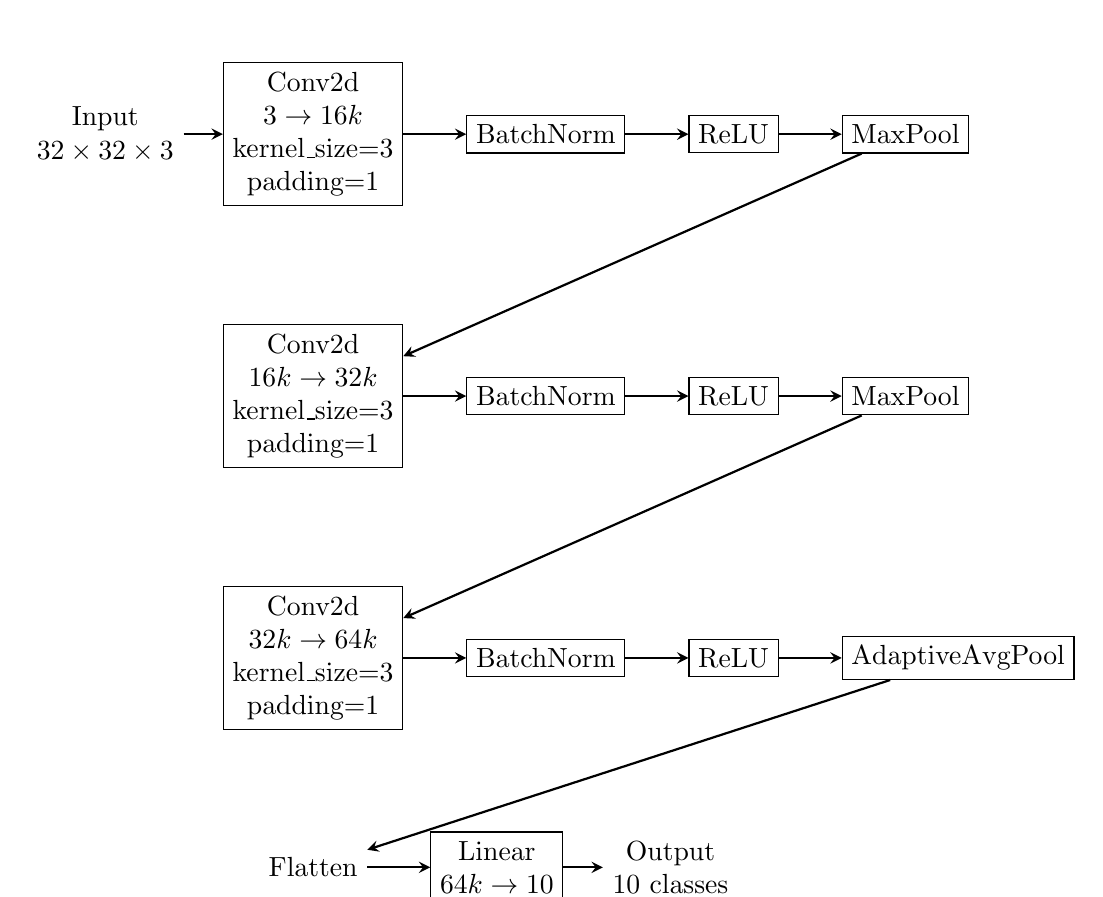
\begin{tikzpicture}[
    node distance=0.8cm,
    conv/.style={draw=black, align=center},
    norm/.style={ draw=black, align=center},
    act/.style={ draw=black, align=center},
    pool/.style={ draw=black, align=center},
    linear/.style={ draw=black, align=center},
    arrow/.style={->, thick, >=stealth},
]
    % Block 1
    \node[conv] (conv1) {Conv2d\\$3 \to 16k$\\kernel\_size=3\\padding=1};
    \node[norm, right=of conv1] (bn1) {BatchNorm};
    \node[act, right=of bn1] (relu1) {ReLU};
    \node[pool, right=of relu1] (pool1) {MaxPool};
    
    % Block 2
    \node[conv, below=1.5cm of conv1] (conv2) {Conv2d\\$16k \to 32k$\\kernel\_size=3\\padding=1};
    \node[norm, right=of conv2] (bn2) {BatchNorm};
    \node[act, right=of bn2] (relu2) {ReLU};
    \node[pool, right=of relu2] (pool2) {MaxPool};
    
    % Block 3
    \node[conv, below=1.5cm of conv2] (conv3) {Conv2d\\$32k \to 64k$\\kernel\_size=3\\padding=1};
    \node[norm, right=of conv3] (bn3) {BatchNorm};
    \node[act, right=of bn3] (relu3) {ReLU};
    \node[pool, right=of relu3] (pool3) {AdaptiveAvgPool};
    
    % Final layers
    \node[below=1.5cm of conv3, minimum width=1.2cm] (flat) {Flatten};
    \node[linear, right=of flat] (linear) {Linear\\$64k \to 10$};
    
    % Arrows within blocks
    \draw[arrow] (conv1) -- (bn1);
    \draw[arrow] (bn1) -- (relu1);
    \draw[arrow] (relu1) -- (pool1);
    
    \draw[arrow] (conv2) -- (bn2);
    \draw[arrow] (bn2) -- (relu2);
    \draw[arrow] (relu2) -- (pool2);
    
    \draw[arrow] (conv3) -- (bn3);
    \draw[arrow] (bn3) -- (relu3);
    \draw[arrow] (relu3) -- (pool3);
    
    \draw[arrow] (pool3) -- (flat);
    \draw[arrow] (flat) -- (linear);
    
    % Vertical connections between blocks
    \draw[arrow] (pool1) -- (conv2);
    \draw[arrow] (pool2) -- (conv3);
    
    % Input
    \node[left=0.5cm of conv1, align=center] (input) {Input\\$32 \times 32 \times 3$};
    \draw[arrow] (input) -- (conv1);
    
    % Output
    \node[right=0.5cm of linear, align=center] (output) {Output\\10 classes};
    \draw[arrow] (linear) -- (output);
\end{tikzpicture}
\caption{Architecture of $\text{ScaledCNN}(k)$.}
\label{fig:scaledcnn}
\end{figure}

The procedure is as follows:

\subsubsection{Hyperparameter Tuning}

A single, medium-sized model is selected. Hyperparameters such as learning rate, weight decay, and momentum are tuned on the noisy training set and evaluated on the clean validation set with Optuna.

These hyperparameters are then fixed for all other values of $k$.

\subsubsection{Training}

A series of models with varying $k$ (1, 2, 4, 8, 16, 32, 64) are trained from scratch on the noisy training set and evaluated on the clean validation set for a fixed, large number of epochs to ensure all models including large ones have sufficient time to interpolate the data.

\subsubsection{Data Collection}

For each trained model $k$, the final test error on the 10,000 image clean test set is recorded. This data is used to plot the Test Error vs. Model Capacity, which is hypothesized to reveal the double descent curve.

\subsection{Analysis}

To conduct a thorough analysis, we will be using two different methods:

\subsubsection{Statistical Significance}

TODO

\subsubsection{Error Analysis}

A full $10\times10$ confusion matrix will be generated for the three key models: the classical SVM baseline, the medium-sized CNN (at error peak), and the over-parametrized CNN (in the second descent).

These matrices will be qualitatively analyzed to identify patterns such as identifying inter-class confusions.

\subsection{Results and Analysis}

FOO

\clearpage
\bibliographystyle{plain}
\bibliography{bibliography}

\end{document}